\chapter{Probing Results}
\label{chap:results}
In this section we will analyze and discuss the results from the probing experiments. Since the overall distribution of properties across layers follows a similar pattern across models, we will first focus on the distribution on \ti{bert-base-uncased}, then discuss the effects of fine-tuning in the following section.

\section{Distribution of Ranking Properties}
Firstly, a general trend we can observe across tasks, is an increase in both compression and accuracy over the first couple of layers up to layer 4-6, suggesting that ranking concepts arise mostly in the mid-range of layers. Then, after a peak at some mid to upper level layer, we observe a constant decrease until the last layer. It is notable that accuracy appears to exhibit a less stable curve, with sudden peaks and drops in between adjacent layers, especially in the case of coreference resolution (COREF) and semantic similarity (SEM) \autoref{fig:sem_sim_coref}. This observation coincides with \cite{voita-titov-2020-information} findings, that MDL and as a consequence compression, are a more reliable measure for probing than accuracy.

For the most part, based on compression, ranking properties can be decoded more efficiently from our trained models than from the random baseline, meaning the probe model is not solely adapting to the task, but instead leveraging information present in the pre-trained representations.

We can further observe that the difference in compression between early layers and the peak value varies depending on the task. This Indicates that some properties are more uniformly distributed across layers, while others are more concentrated at a particular layer. For example, decoding named entities results in similar compression scores from layer 1-11, while SEM shows a distinct peak at layer 4.

\begin{figure}[!h]
    \centering
    \begin{subfigure}{\textwidth}
        \centering
        \makebox[\textwidth][c]{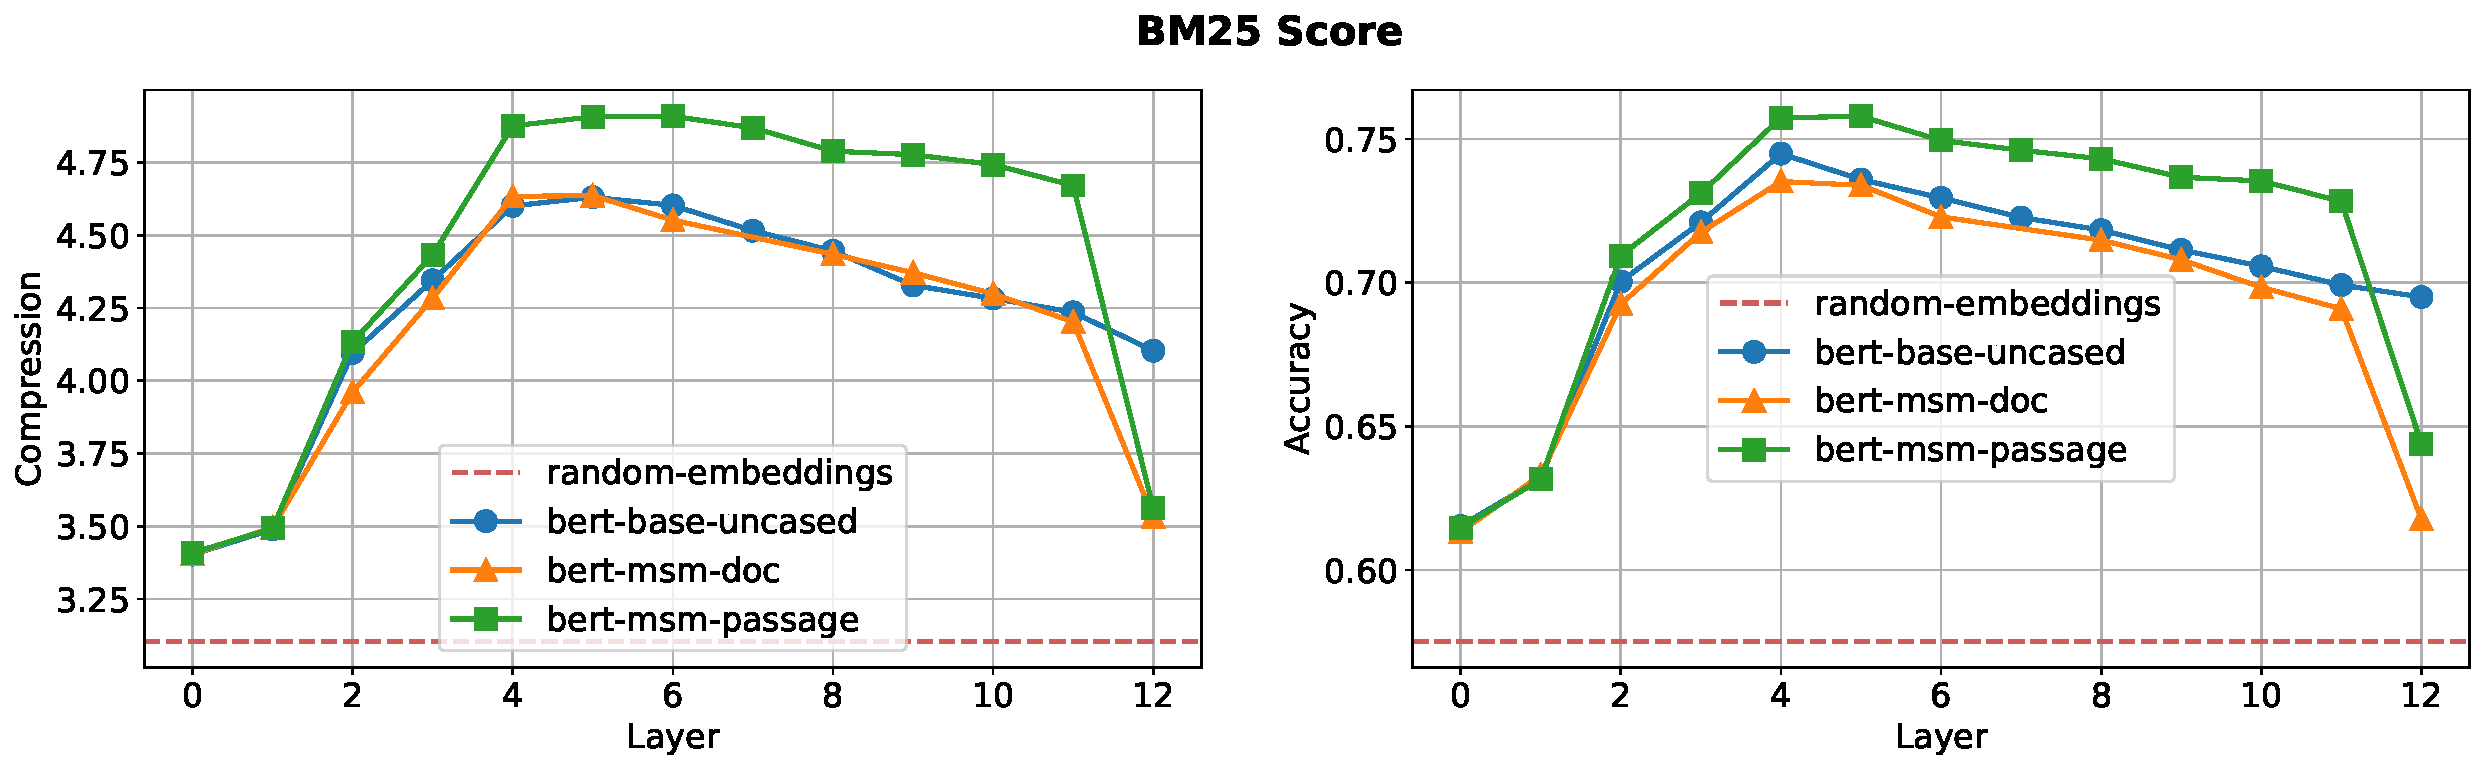
\includegraphics[width=1.2\textwidth]{gfx/probing/bm25}}
    \end{subfigure}

    \begin{subfigure}{\textwidth}
        \centering
        \makebox[\textwidth][c]{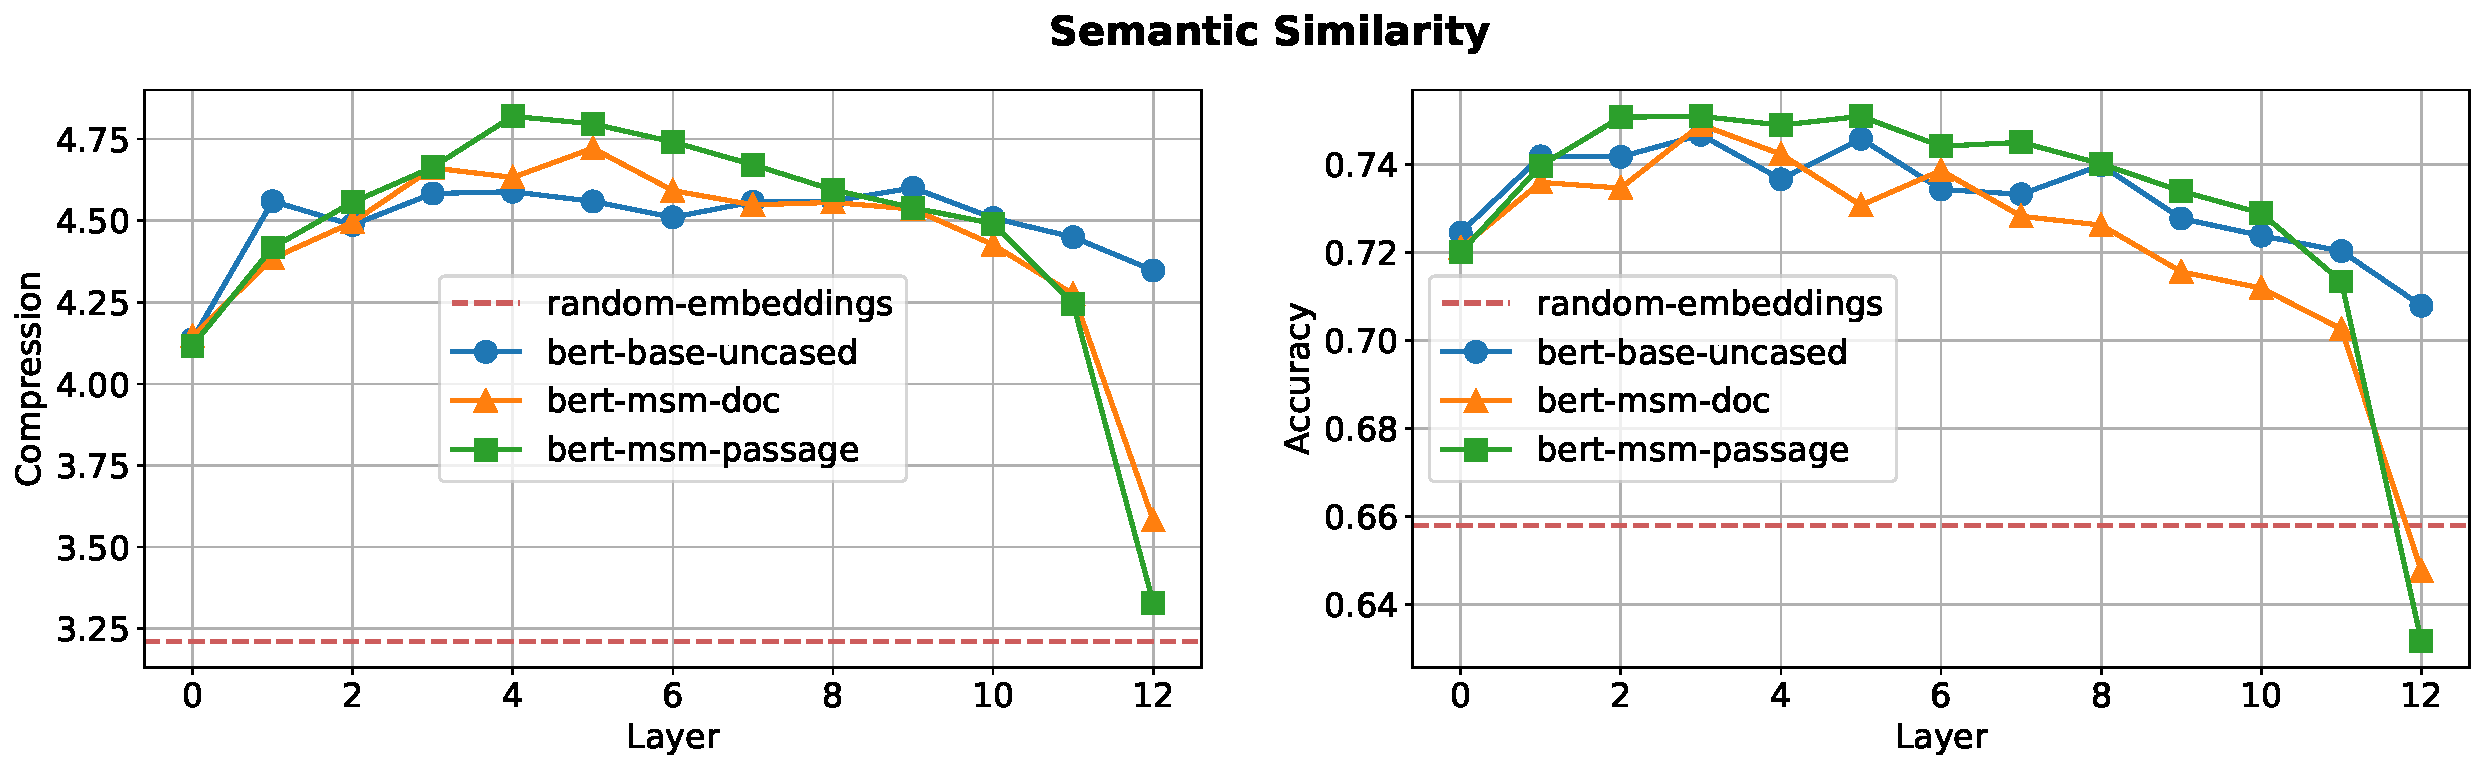
\includegraphics[width=1.2\textwidth]{gfx/probing/sem_sim}}
    \end{subfigure}

    \begin{subfigure}{\textwidth}
        \centering
        \makebox[\textwidth][c]{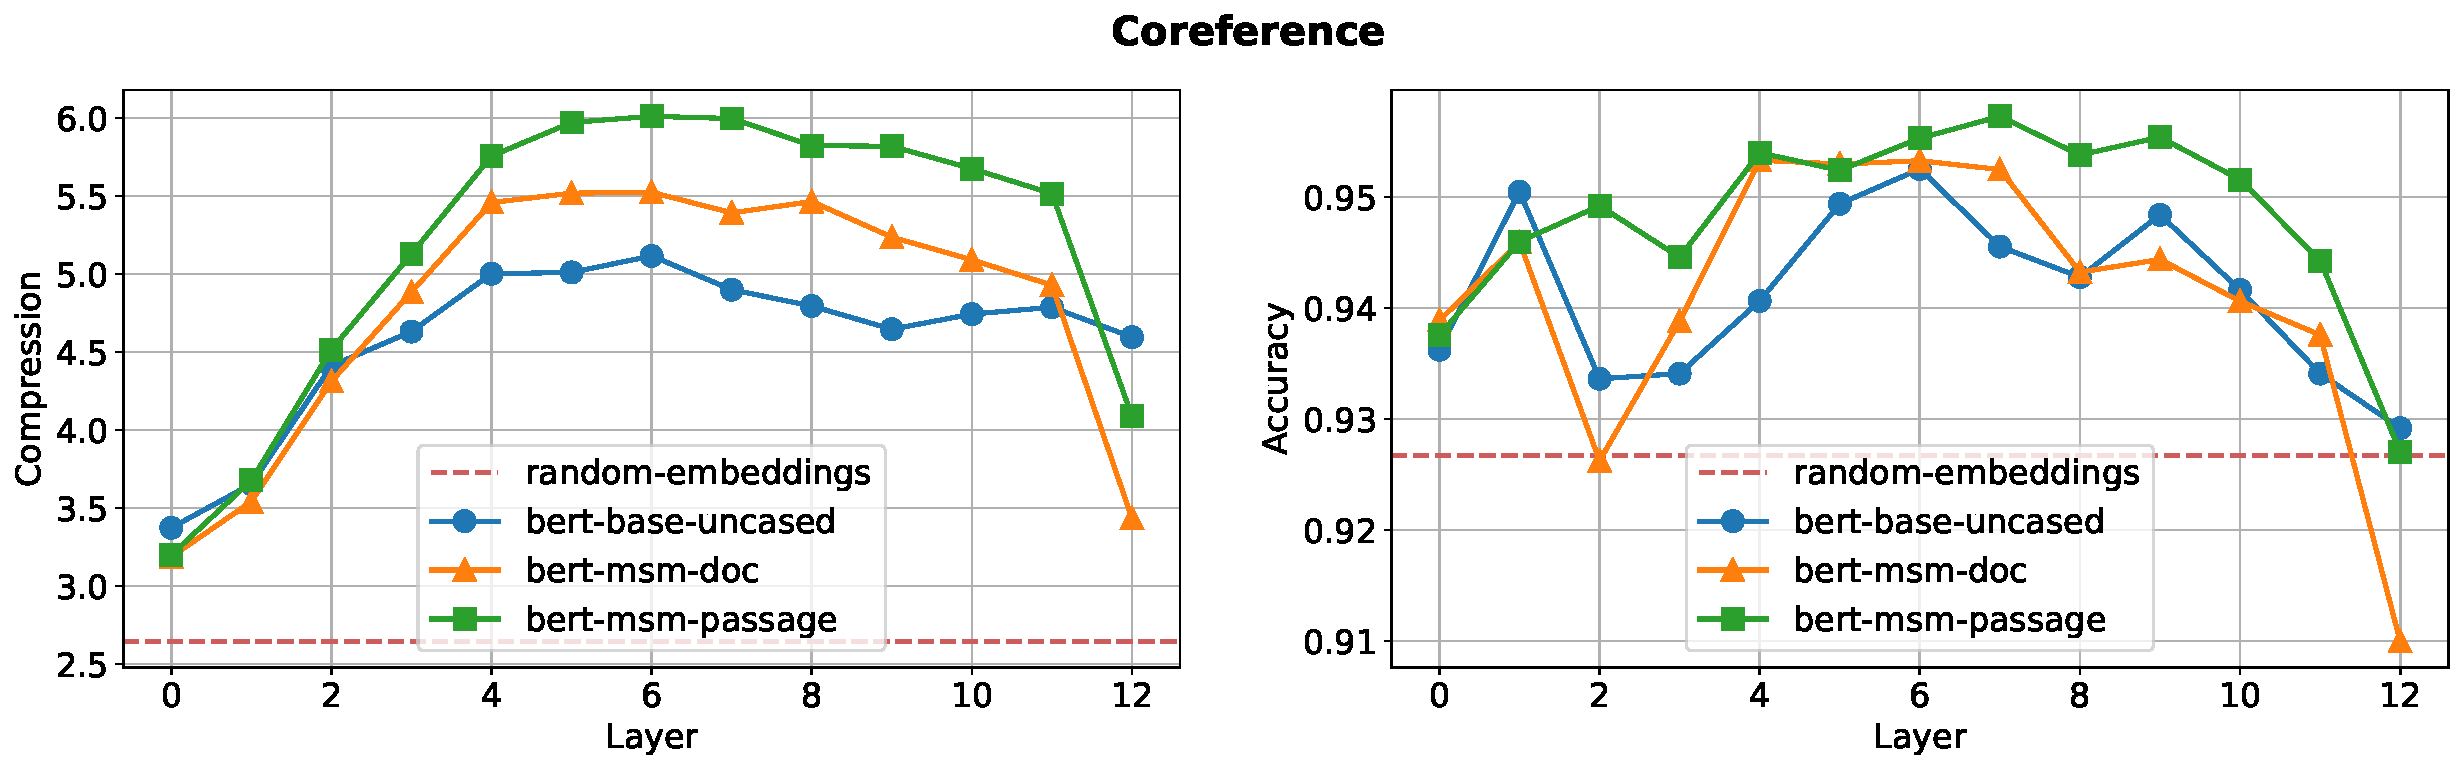
\includegraphics[width=1.2\textwidth]{gfx/probing/coref}}
    \end{subfigure}

    \caption{Layer to probing score for BM25, semantic similarity and coreference properties. We report accuracy on the test set.}
    \label{fig:sem_sim_coref}
\end{figure}

\begin{figure}[!h]
    \centering
    \begin{subfigure}{\textwidth}
        \centering
        \makebox[\textwidth][c]{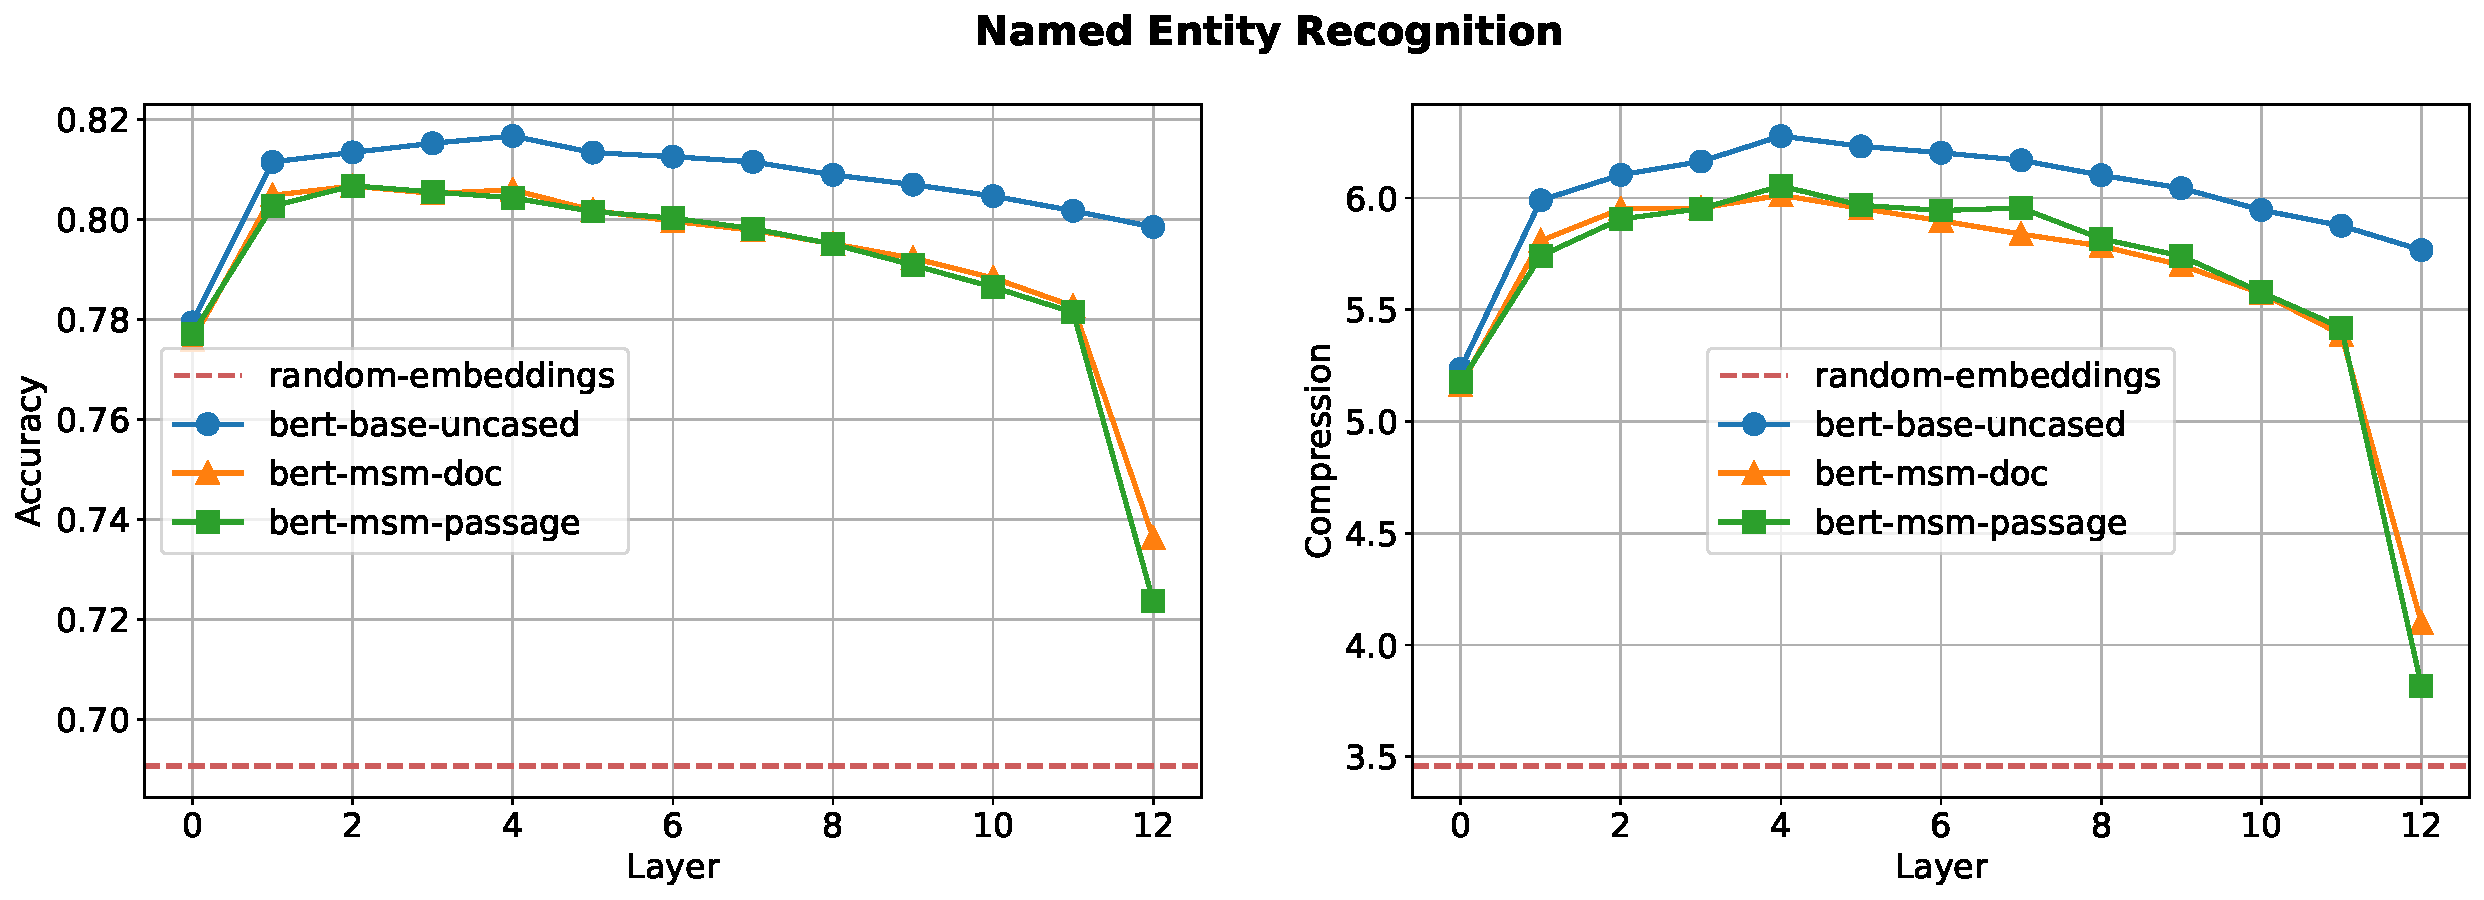
\includegraphics[width=1.2\textwidth]{gfx/probing/ner}}
    \end{subfigure}

    \begin{subfigure}{\textwidth}
        \centering
        \makebox[\textwidth][c]{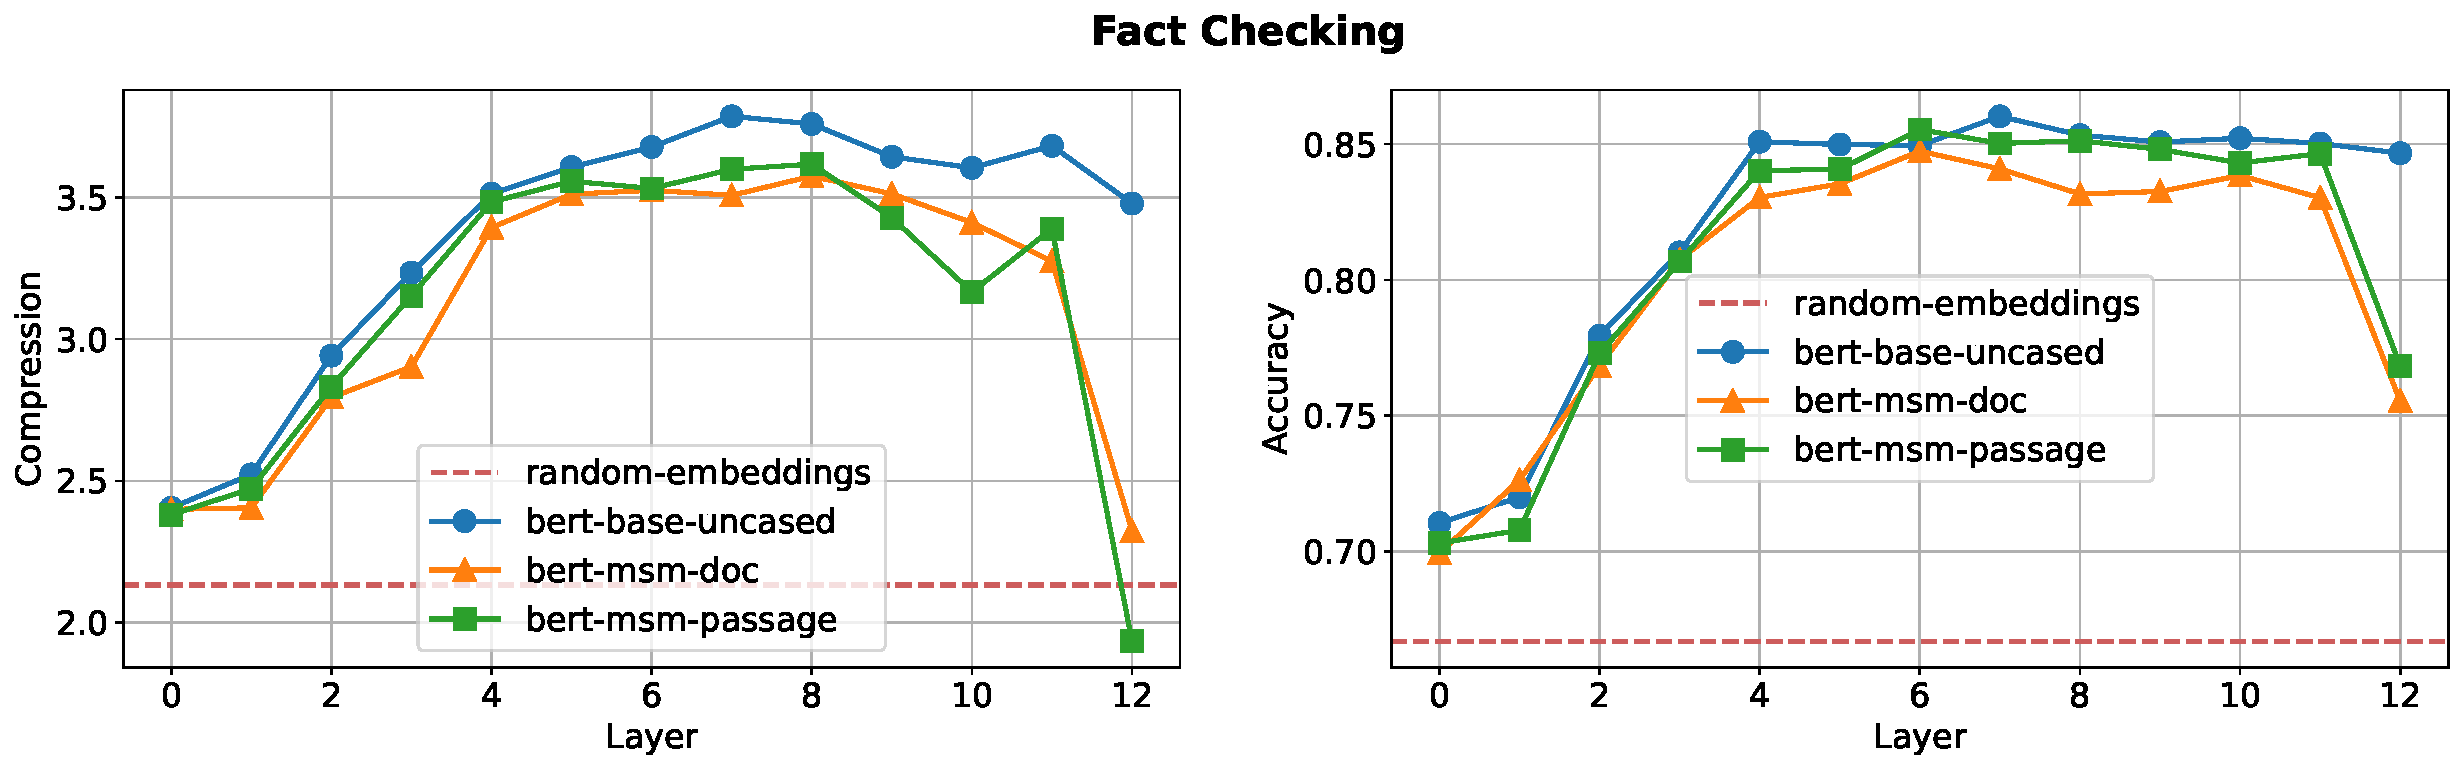
\includegraphics[width=1.2\textwidth]{gfx/probing/fact_check}}
    \end{subfigure}

    \caption{Layer to probing score for NER and fact checking properties. We report accuracy on the test set.}
\end{figure}

To better understand this behavior, we can have a look at the row-normalized heatmap in \autoref{fig:heatmap_comp_base} of the \ti{bert-base-uncased} model. We can see that COREF and fact checking strongly center around layers 4-7 and 6-9 respectively, with fact checking showing a slightly wider spread. While BM25 exhibits a similar pattern, it is less focused around a particular layer, but instead more evenly distributed from layer 4-6. SEM and NER on the other hand look almost identical, with a rather flat distribution that is more prominent in early layers 1-4.

\begin{figure}[!h]
    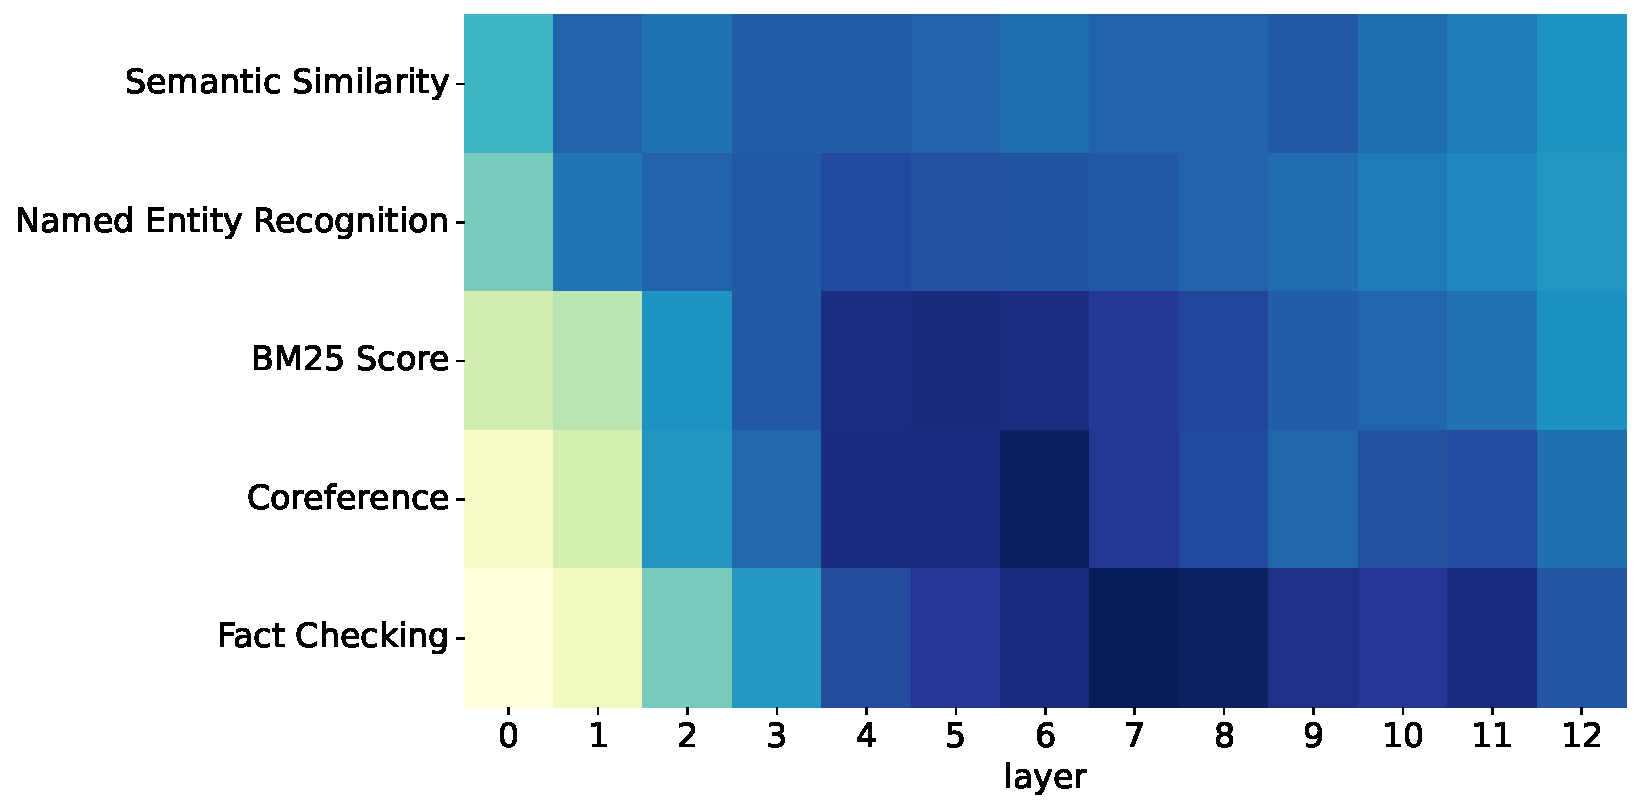
\includegraphics[width=\textwidth]{gfx/probing/heatmap_compression_base}
    \caption{\ti{bert-base-uncased}: compression as a function of task and layer, row-normalized. Darker colors represent higher values.}
    \label{fig:heatmap_comp_base}

    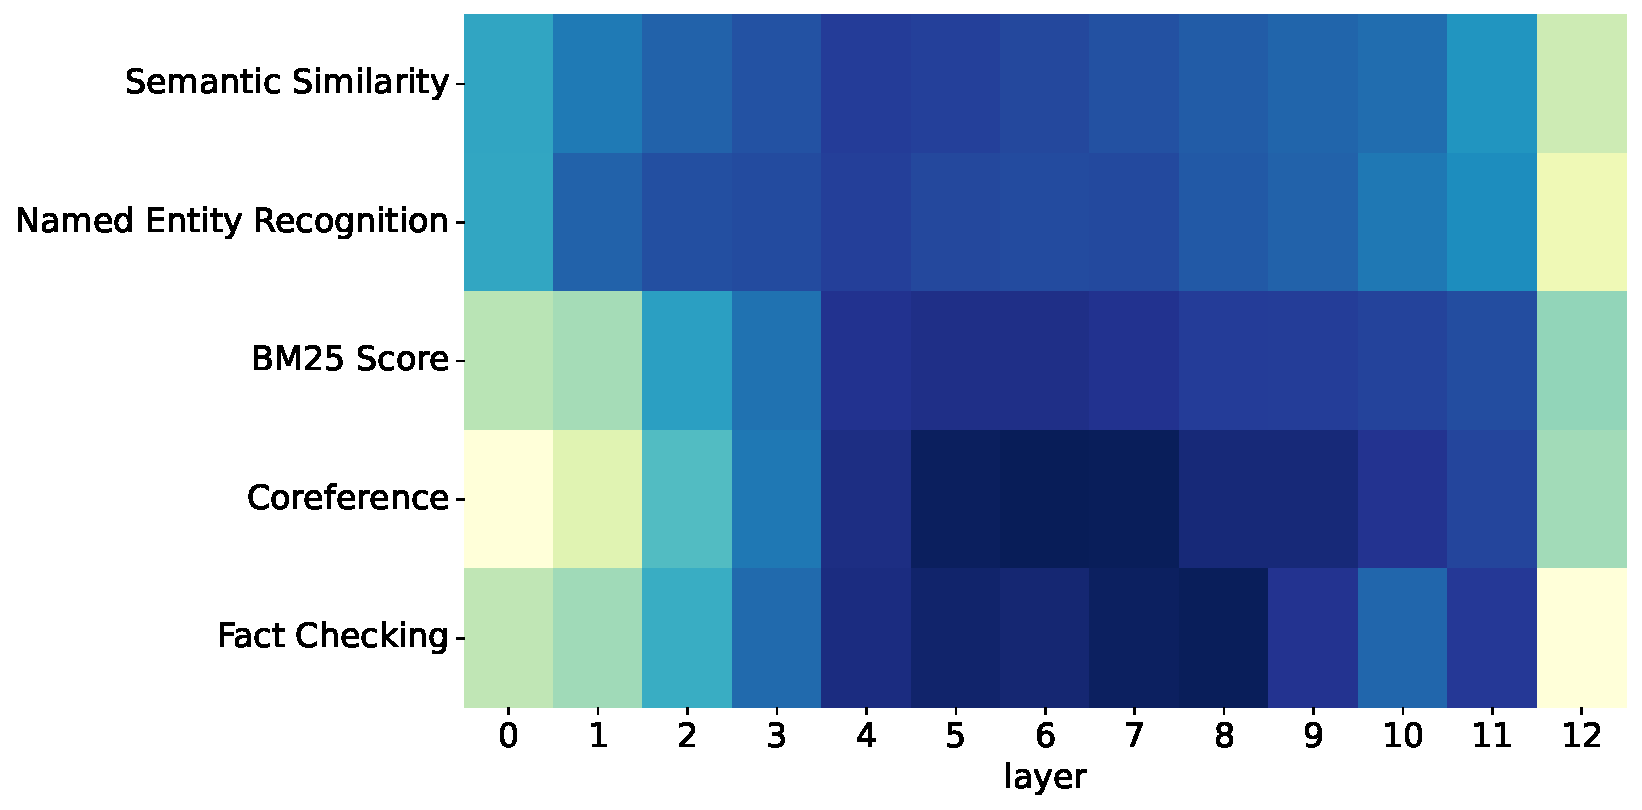
\includegraphics[width=\textwidth]{gfx/probing/heatmap_compression_passage}
    \caption{\ti{bert-msm-passage} - compression as a function of task and layer, row-normalized. Darker colors represent higher values.}
    \label{fig:heatmap_comp_passage}
\end{figure}

When considering that COREF and fact checking are both tasks that require higher level semantics, based on the observation in \cite{tenney-etal-2019-bert}, it makes sense that both distributions are leaning more towards mid to upper layers. On the other hand, based on this, we would expect a lower level concept such as SEM to be mostly present in early layers. Especially since it is a property that can already be captured by non-contextual word embeddings. However, except a slight peak at layer 1, we observe it to be more evenly spread across layers. We hypothesize that, as a fundamental concept which higher level tasks build on, it's a property of the embedding space that needs to be preserved throughout the whole model.

Further, even though NER appears to be a higher level concept than SEM at first, considering that similar categories of entities are likely grouped together in the embedding space \cite{DBLP:journals/corr/abs-1301-3781, pennington2014glove}, a relation to SEM property becomes apparent. Given that NER requires us to predict \ti{categories} of entities, it might explain that NER shares a very similar distribution with SEM.

BM25 depends on both local and corpus-level frequency statistics of words. Finding that layers 4-6 are best for inferring BM25 might indicate that some kind of direct term comparison between query and document is modeled within this range of the model. \cite{https://doi.org/10.48550/arxiv.2202.12191} who probe BERT for IDF, find that the IDF property is present in early layers and constantly decreases up to the final layer. However, unlike IDF, BM25 also encodes term frequency and considers the length of a document, supporting the idea that local interactions are more prominent in the mid-layers, while corpus level statistics are encoded more evenly across the model.

Finally, since compression is a relative measure that compares MDL to the MDL of a uniform encoding, it is possible to compare it \ti{between} tasks. For this, we show absolute compression values in \autoref{fig:abs_heatmap_comp_base}. Firstly, the highest compression can be measured for NER with values $>6$. Further, a compression around $4.5$ is achieved for BM25, SEM and COREF, with COREF showing some peaks closer to $5$. In contrast, for fact checking, we barely reach a compression of $>3.5$. These findings indicate that NER is the most easily extractable property from the pre-trained base model, while fact checking appears to be the hardest.

\begin{figure}[!h]
    \centering
    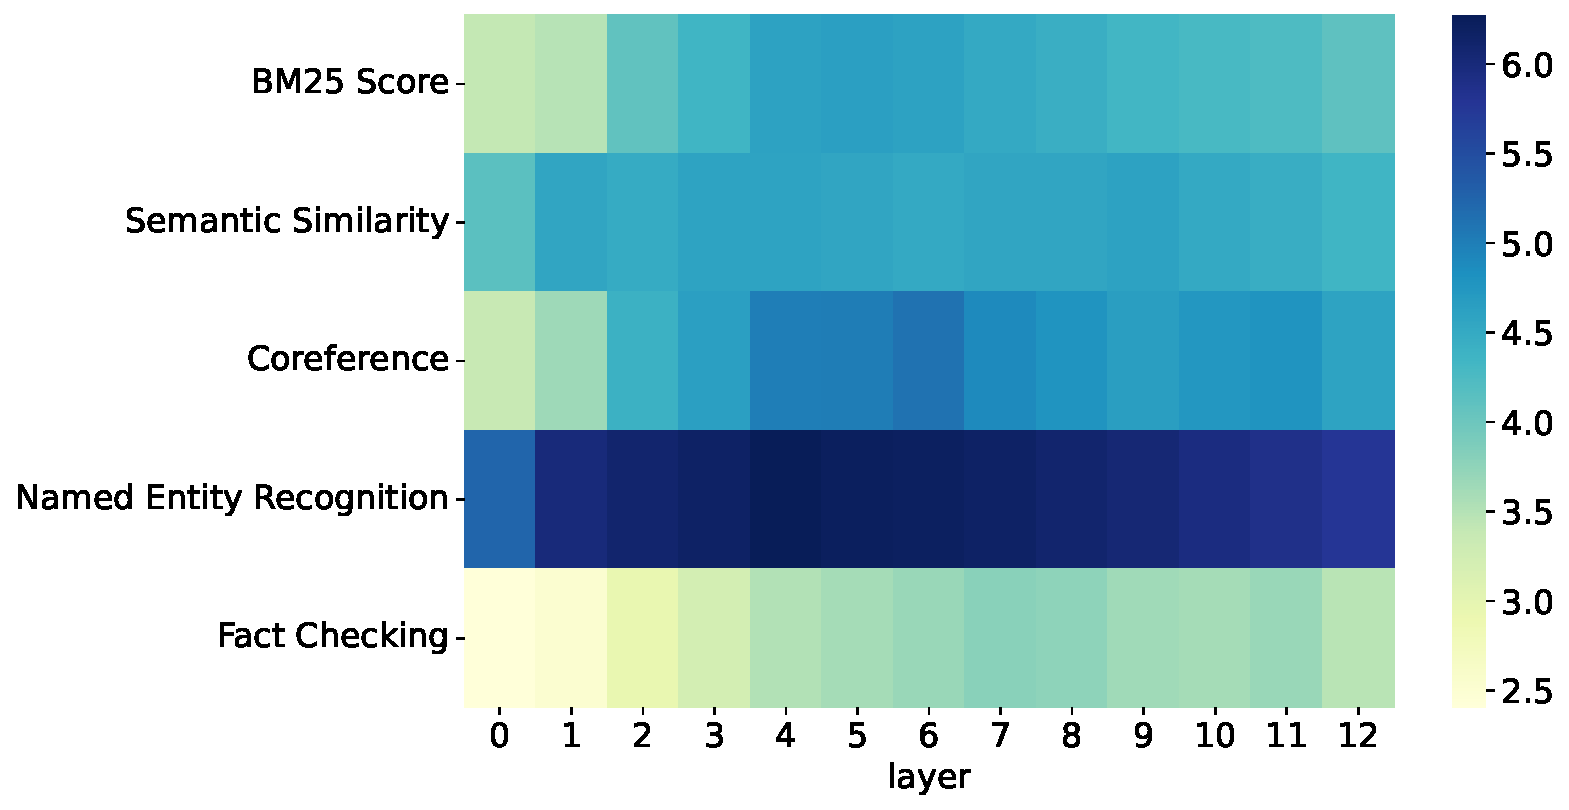
\includegraphics[width=\textwidth]{gfx/probing/abs_heatmap_compression_base}
    \caption{\ti{bert-base-uncased} - compression as a function of task and layer, absolute values.}
    \label{fig:abs_heatmap_comp_base}

    \centering
    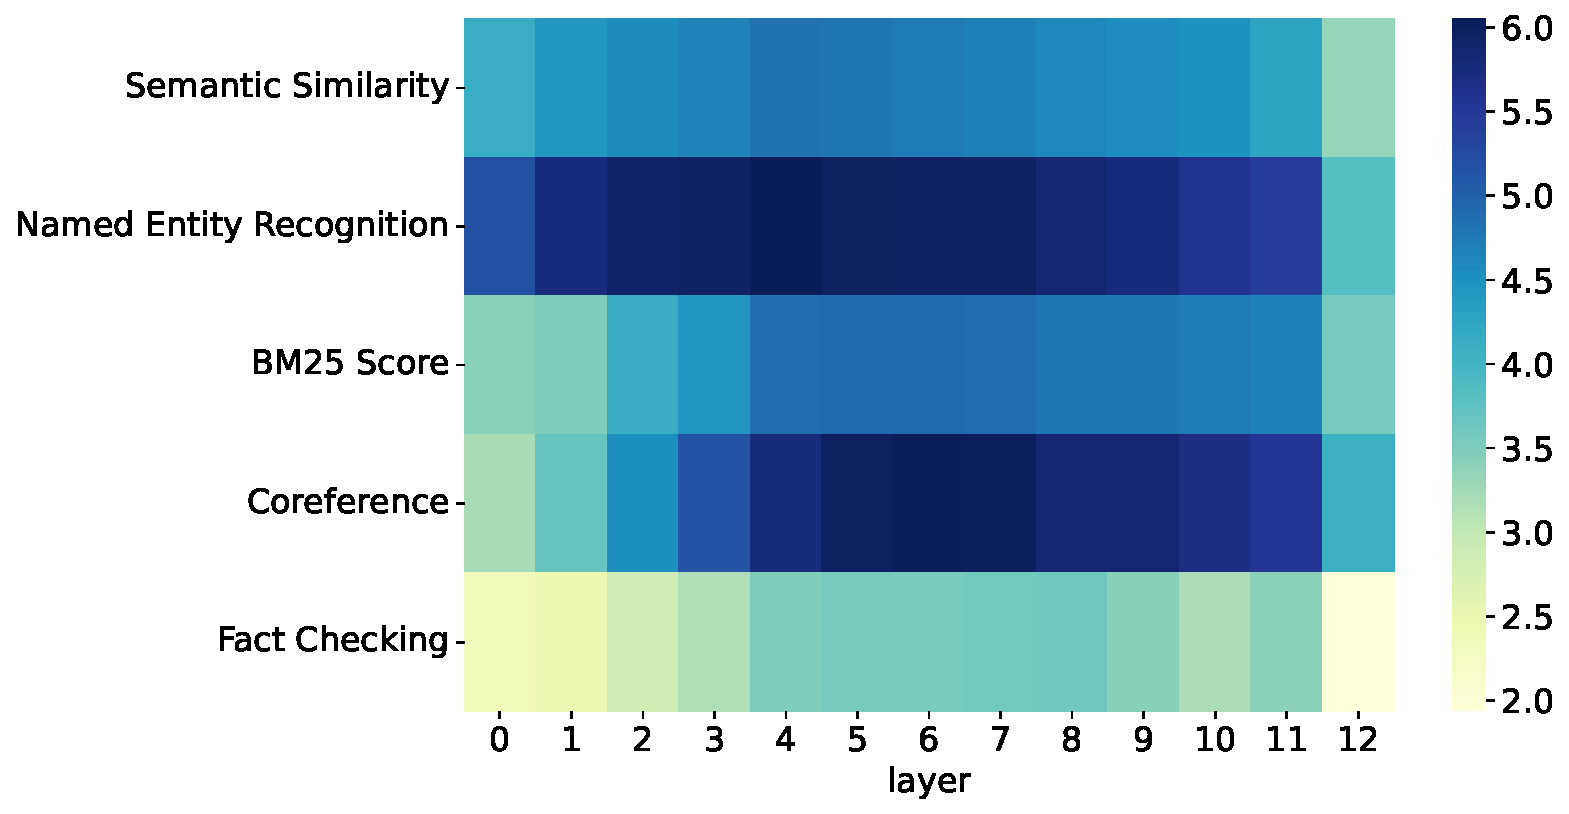
\includegraphics[width=\textwidth]{gfx/probing/abs_heatmap_compression_passage}
    \caption{\ti{bert-msm-passage} - compression as a function of task and layer, absolute values.}
    \label{fig:abs_heatmap_comp_passage}
\end{figure}

\section{Effects of Fine-tuning for Ranking}
First of all, we can observe that for BM25, SEM and COREF resolution, the \ti{bert-msm-passage} representations result in higher compression scores for most layers, suggesting that the extractability of these properties indeed increases through fine-tuning for ranking. Whereas this holds true for \ti{bert-msm-doc} in COREF, for the other two tasks we can observe values closer to \ti{bert-base-uncased}. Moreover, the difference starts to first become apparent around layer 2-3 and begins to increase from there on. This coincides with \cite{merchant-etal-2020-happens}, who find that a change in BERT's representations primarily occurs in the upper layers when fine-tuning.

Surprisingly, for both NER and fact checking, \ti{bert-base-uncased} preserves most of the property while the fine-tuned versions appear to lose some of it. However, this difference also grows with increasing depth.

Another pattern resulting from fine-tuning that we can observe, is a sudden drop in compression at the last layer across all tasks. This might be a sign that through fine-tuning, the final layer becomes more specialized and as a result loses some of the general linguistic knowledge that has been acquired during pre-training. This is also supported by \cite{merchant-etal-2020-happens}.

We can gain further insights on how fine-tuning affects BERT's representations by comparing \autoref{fig:heatmap_comp_base} and \autoref{fig:heatmap_comp_passage}. For SEM, we can see that after fine-tuning, the property's distribution seems to center more around layer 4 and fade out gradually to both sides. In contrast, the pre-trained representations exhibit a more even distribution of the SEM property, with no apparent center. Similarly, the concentration of the NER property in early layers becomes more pronounced.

In contrast, for BM25 a more spread distribution that is shifted towards upper layers can be observed. This behavior is similar to the observations of \cite{https://doi.org/10.48550/arxiv.2202.12191}, who found the IDF property to be more prominent in higher layers of BERT after fine-tuning for ranking. Likewise, COREF related information appears to shift towards higher layers, however with a distribution that concentrates more around a single layer. On the contrary, the fact checking property appears to spread further across layers with fine-tuning.

Lastly, we can use a heatmap of the absolute compression values to visualize how well knowledge w.r.t. different tasks is extractable from \ti{bert-msm-passage}. While it was already recognizable from the line-plots that for the SEM and BM25 properties, \ti{bert-msm-passage} representations achieve higher compression, from \autoref{fig:abs_heatmap_comp_passage} it becomes much more apparent that the COREF property becomes easier to decode from the embeddings than prior fine-tuning with almost double the compression across the board. This might be evidence that matching entities is an important part of a neural ranking model.



